
\documentclass[12pt]{article}
\usepackage{graphicx}
\usepackage{float}
\usepackage[margin=1in]{geometry}
\usepackage{caption}

\begin{document}

\section{Decision Tree Analysis Results}

% Combined Accuracy Distribution
\subsection{Overall Accuracy Distribution}
\begin{figure}[H]
    \centering
    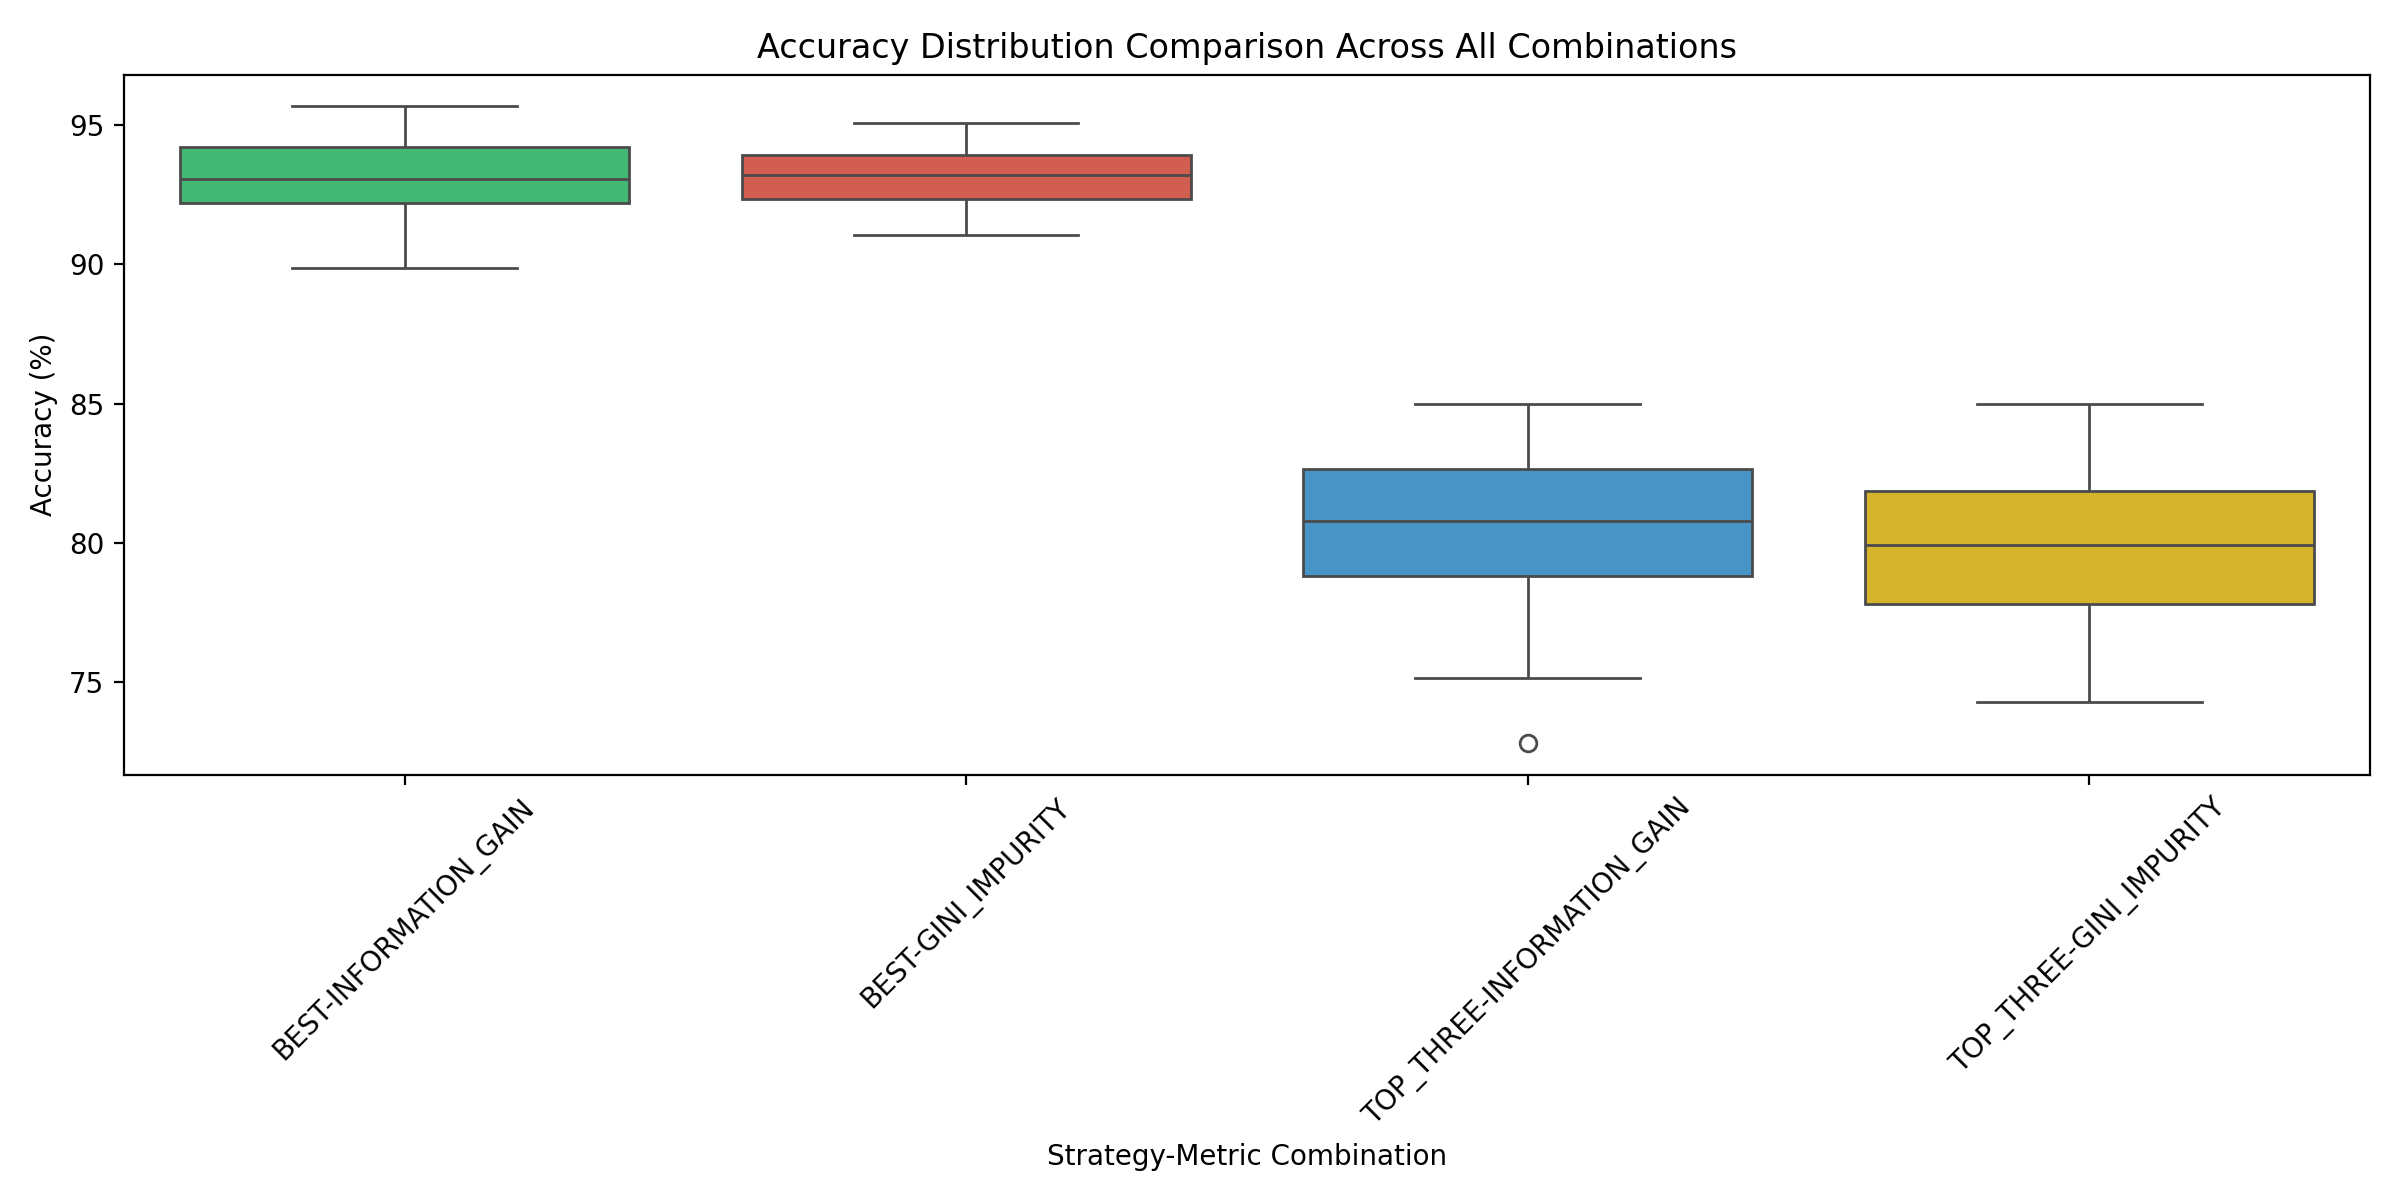
\includegraphics[width=0.9\textwidth]{plots/combined_accuracy_distribution.png}
    \caption{Comparison of accuracy distributions across different strategy and metric combinations.}
    \label{fig:combined-accuracy}
\end{figure}
\newpage

% Combined Confusion Matrices
\subsection{Classification Performance Analysis}
\begin{figure}[H]
    \centering
    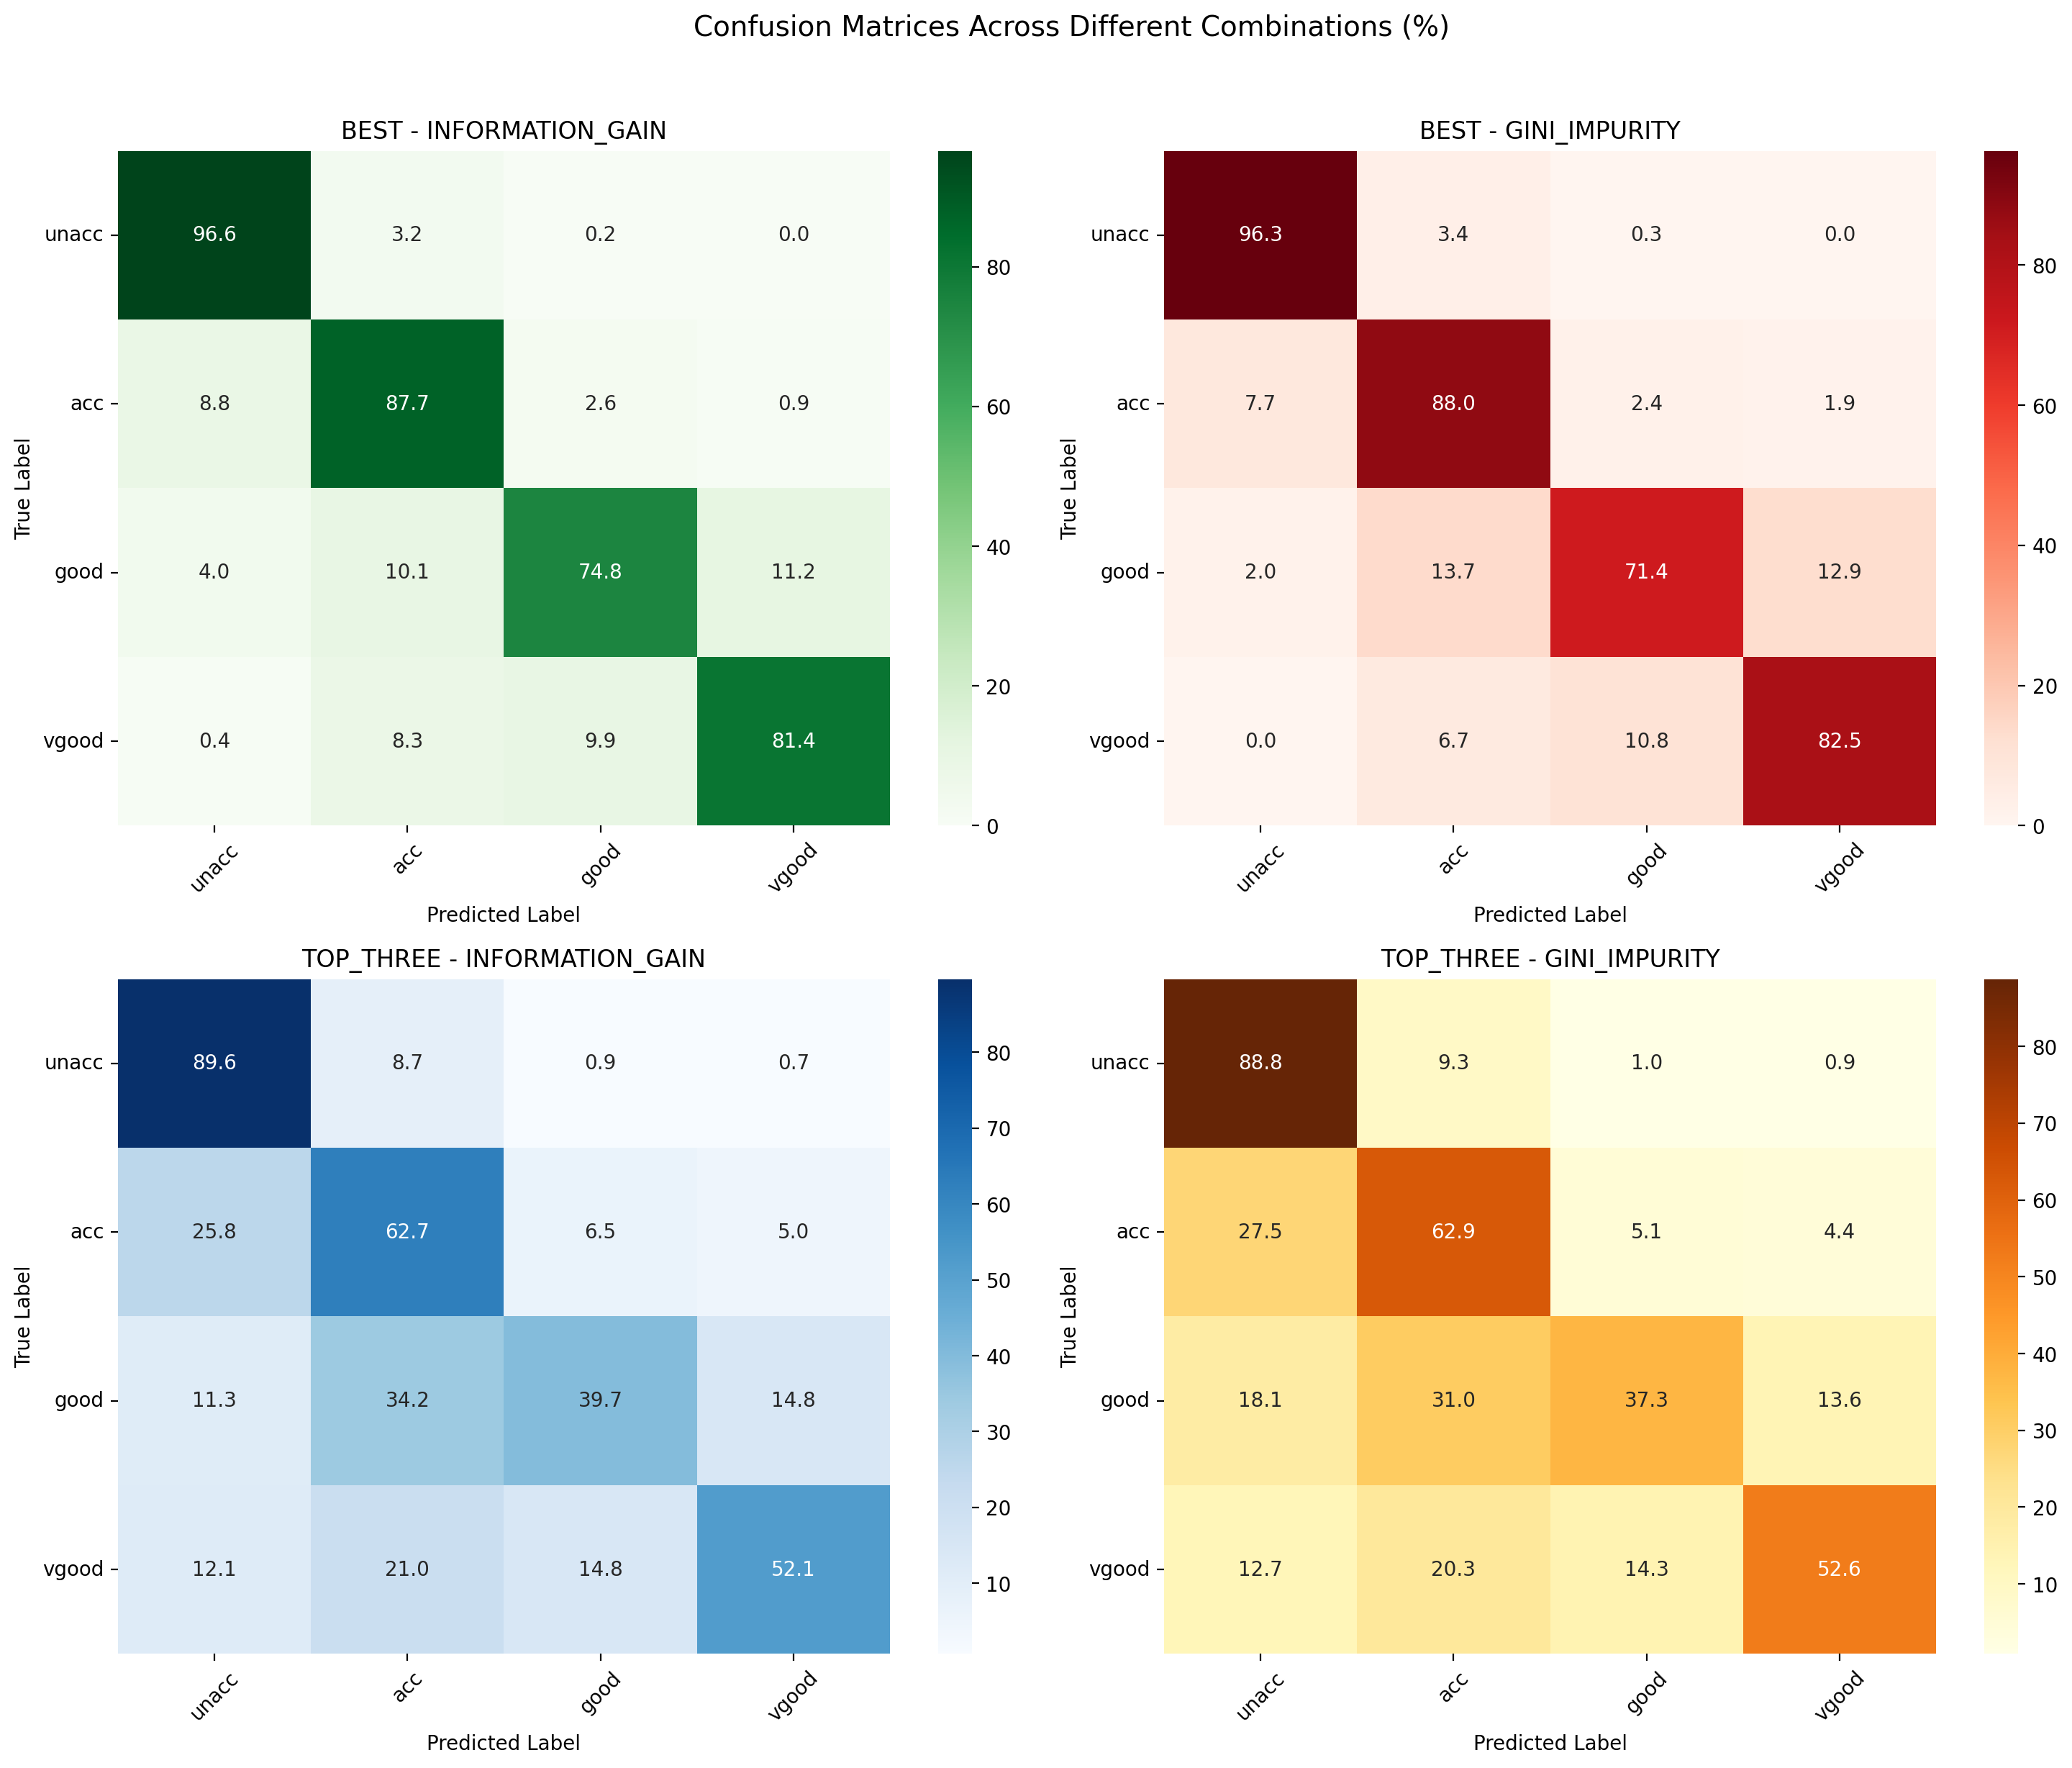
\includegraphics[width=\textwidth]{plots/confusion_matrices_combined.png}
    \caption{Confusion matrices showing classification performance across different strategy-metric combinations. Each subplot uses a different color gradient for better distinction.}
    \label{fig:confusion-matrices}
\end{figure}
\newpage

% Combined Error Rates
\subsection{Error Rate Analysis}
\begin{figure}[H]
    \centering
    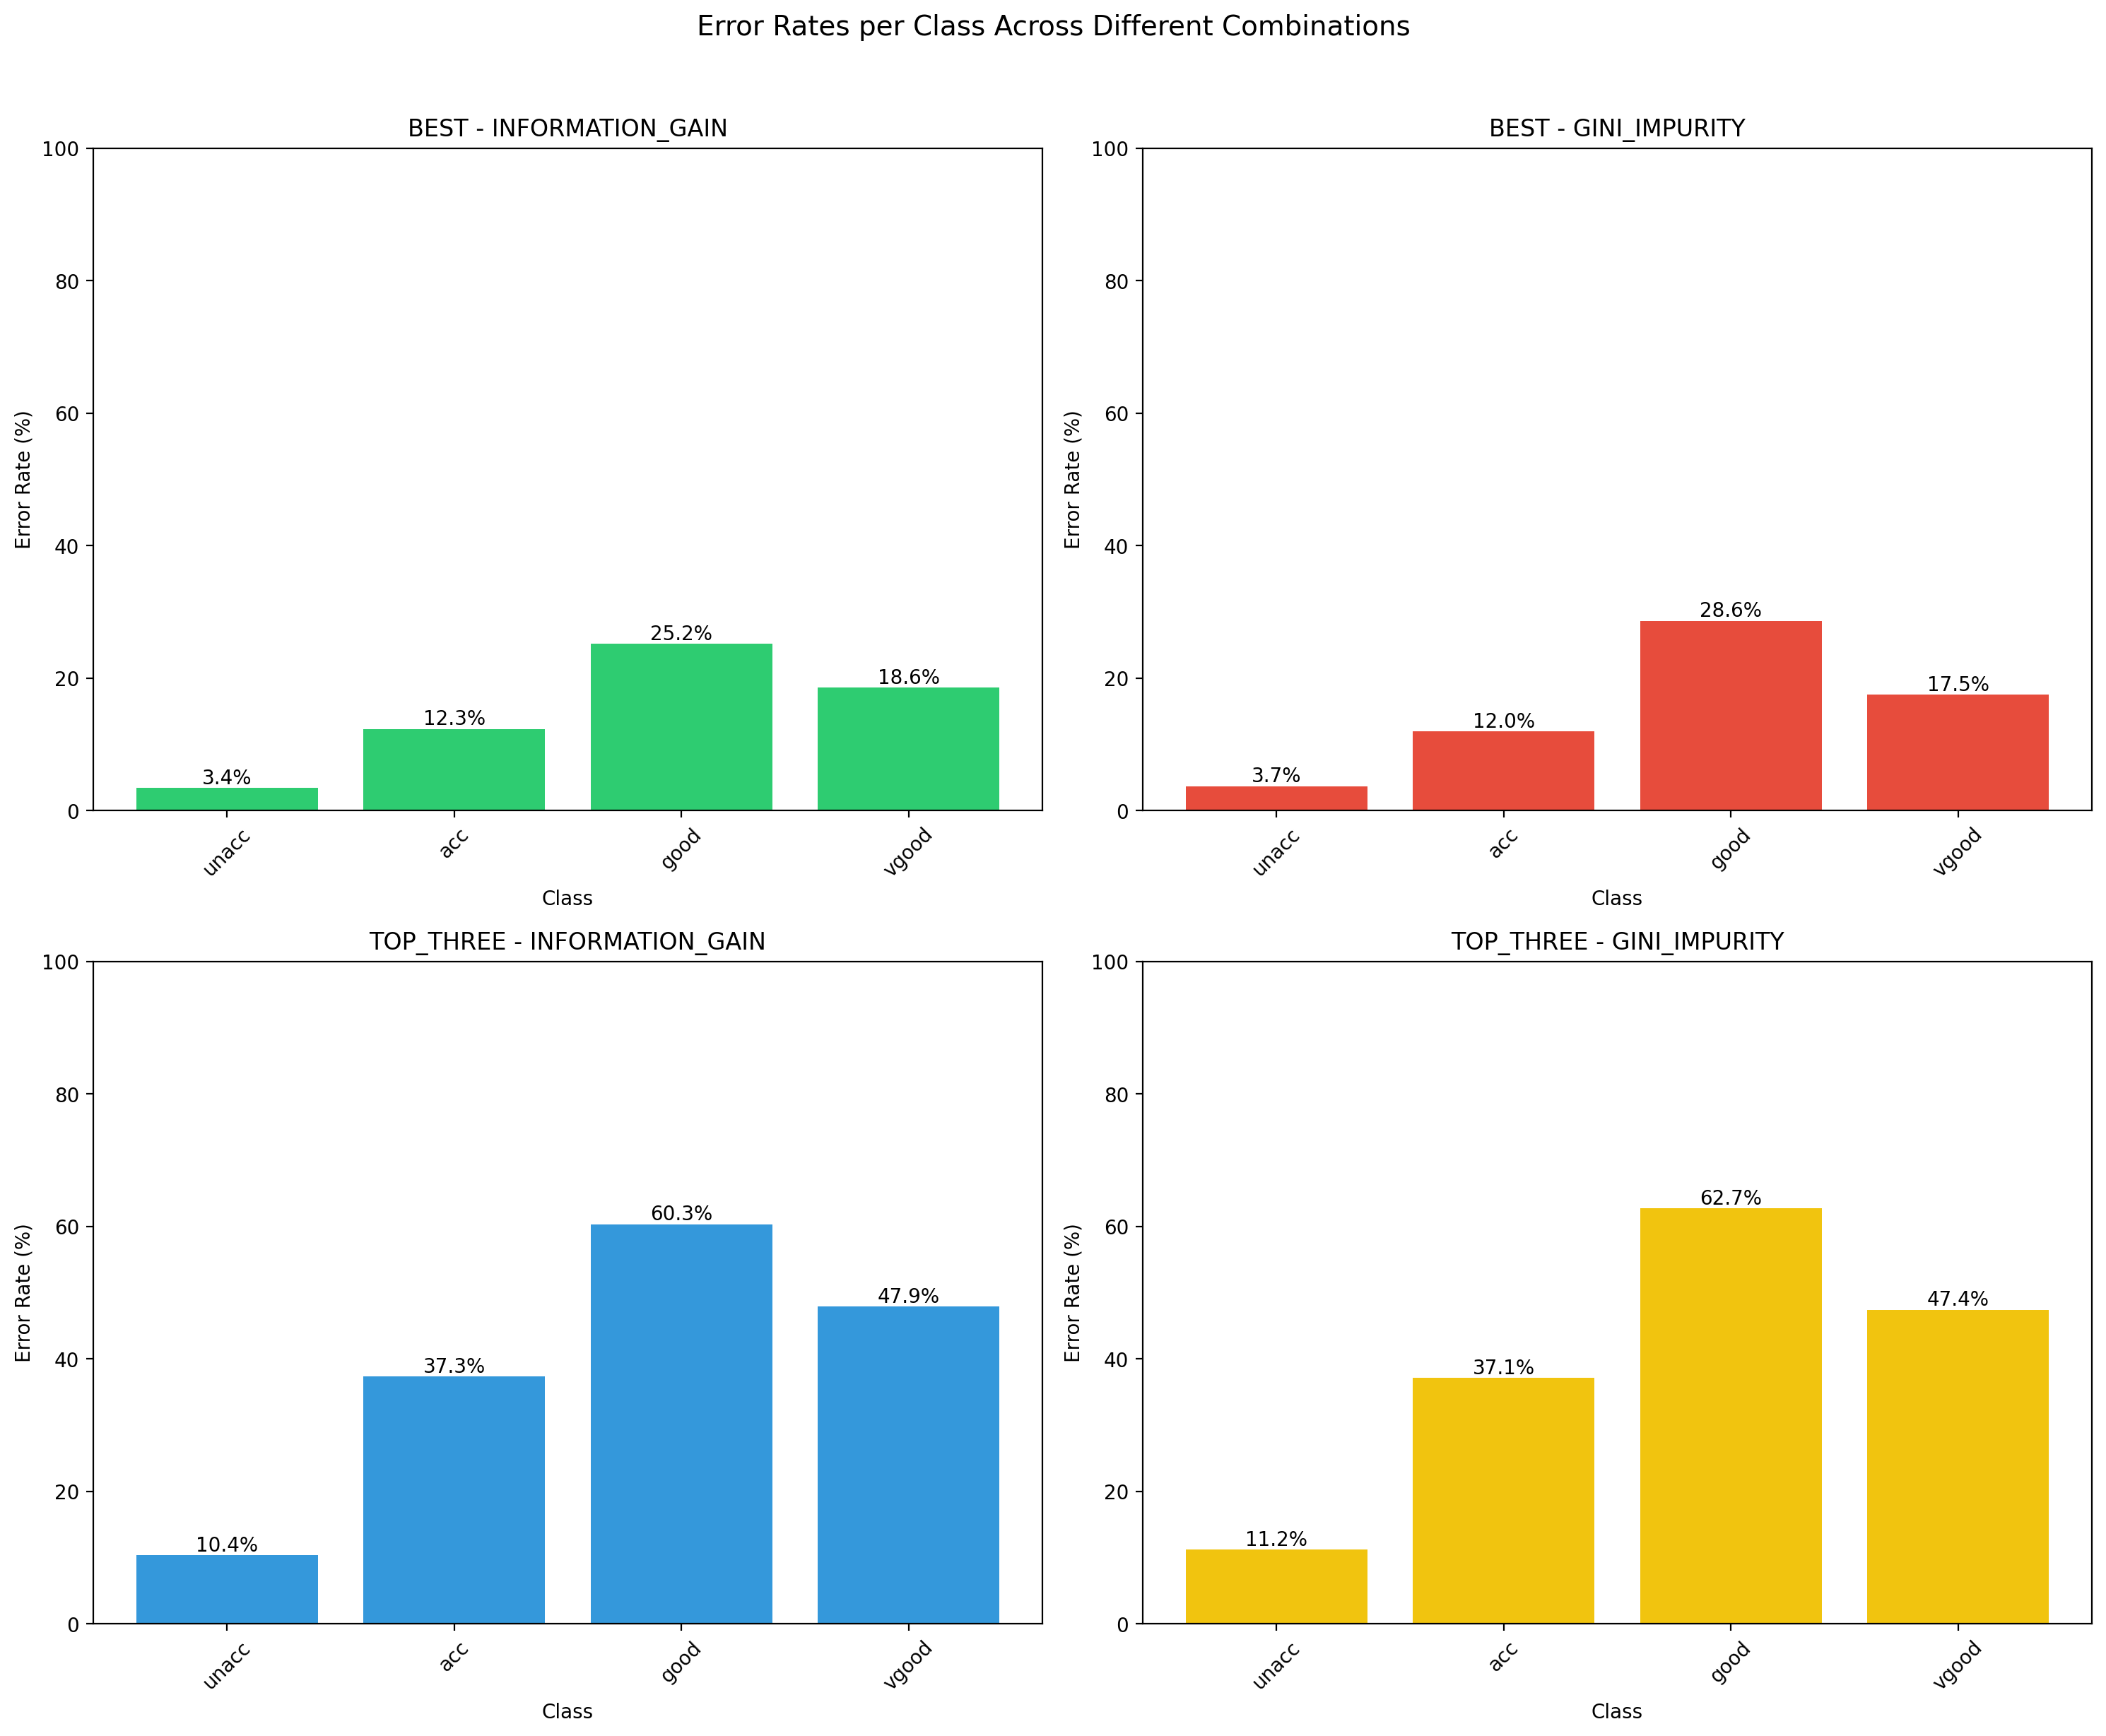
\includegraphics[width=\textwidth]{plots/error_rates_combined.png}
    \caption{Error rates per class across different strategy-metric combinations, showing the misclassification percentages for each category.}
    \label{fig:error-rates}
\end{figure}
\newpage

% Attribute Depths (Individual plots still)
\subsection{Attribute Depth Analysis}
\begin{figure}[H]
    \centering
    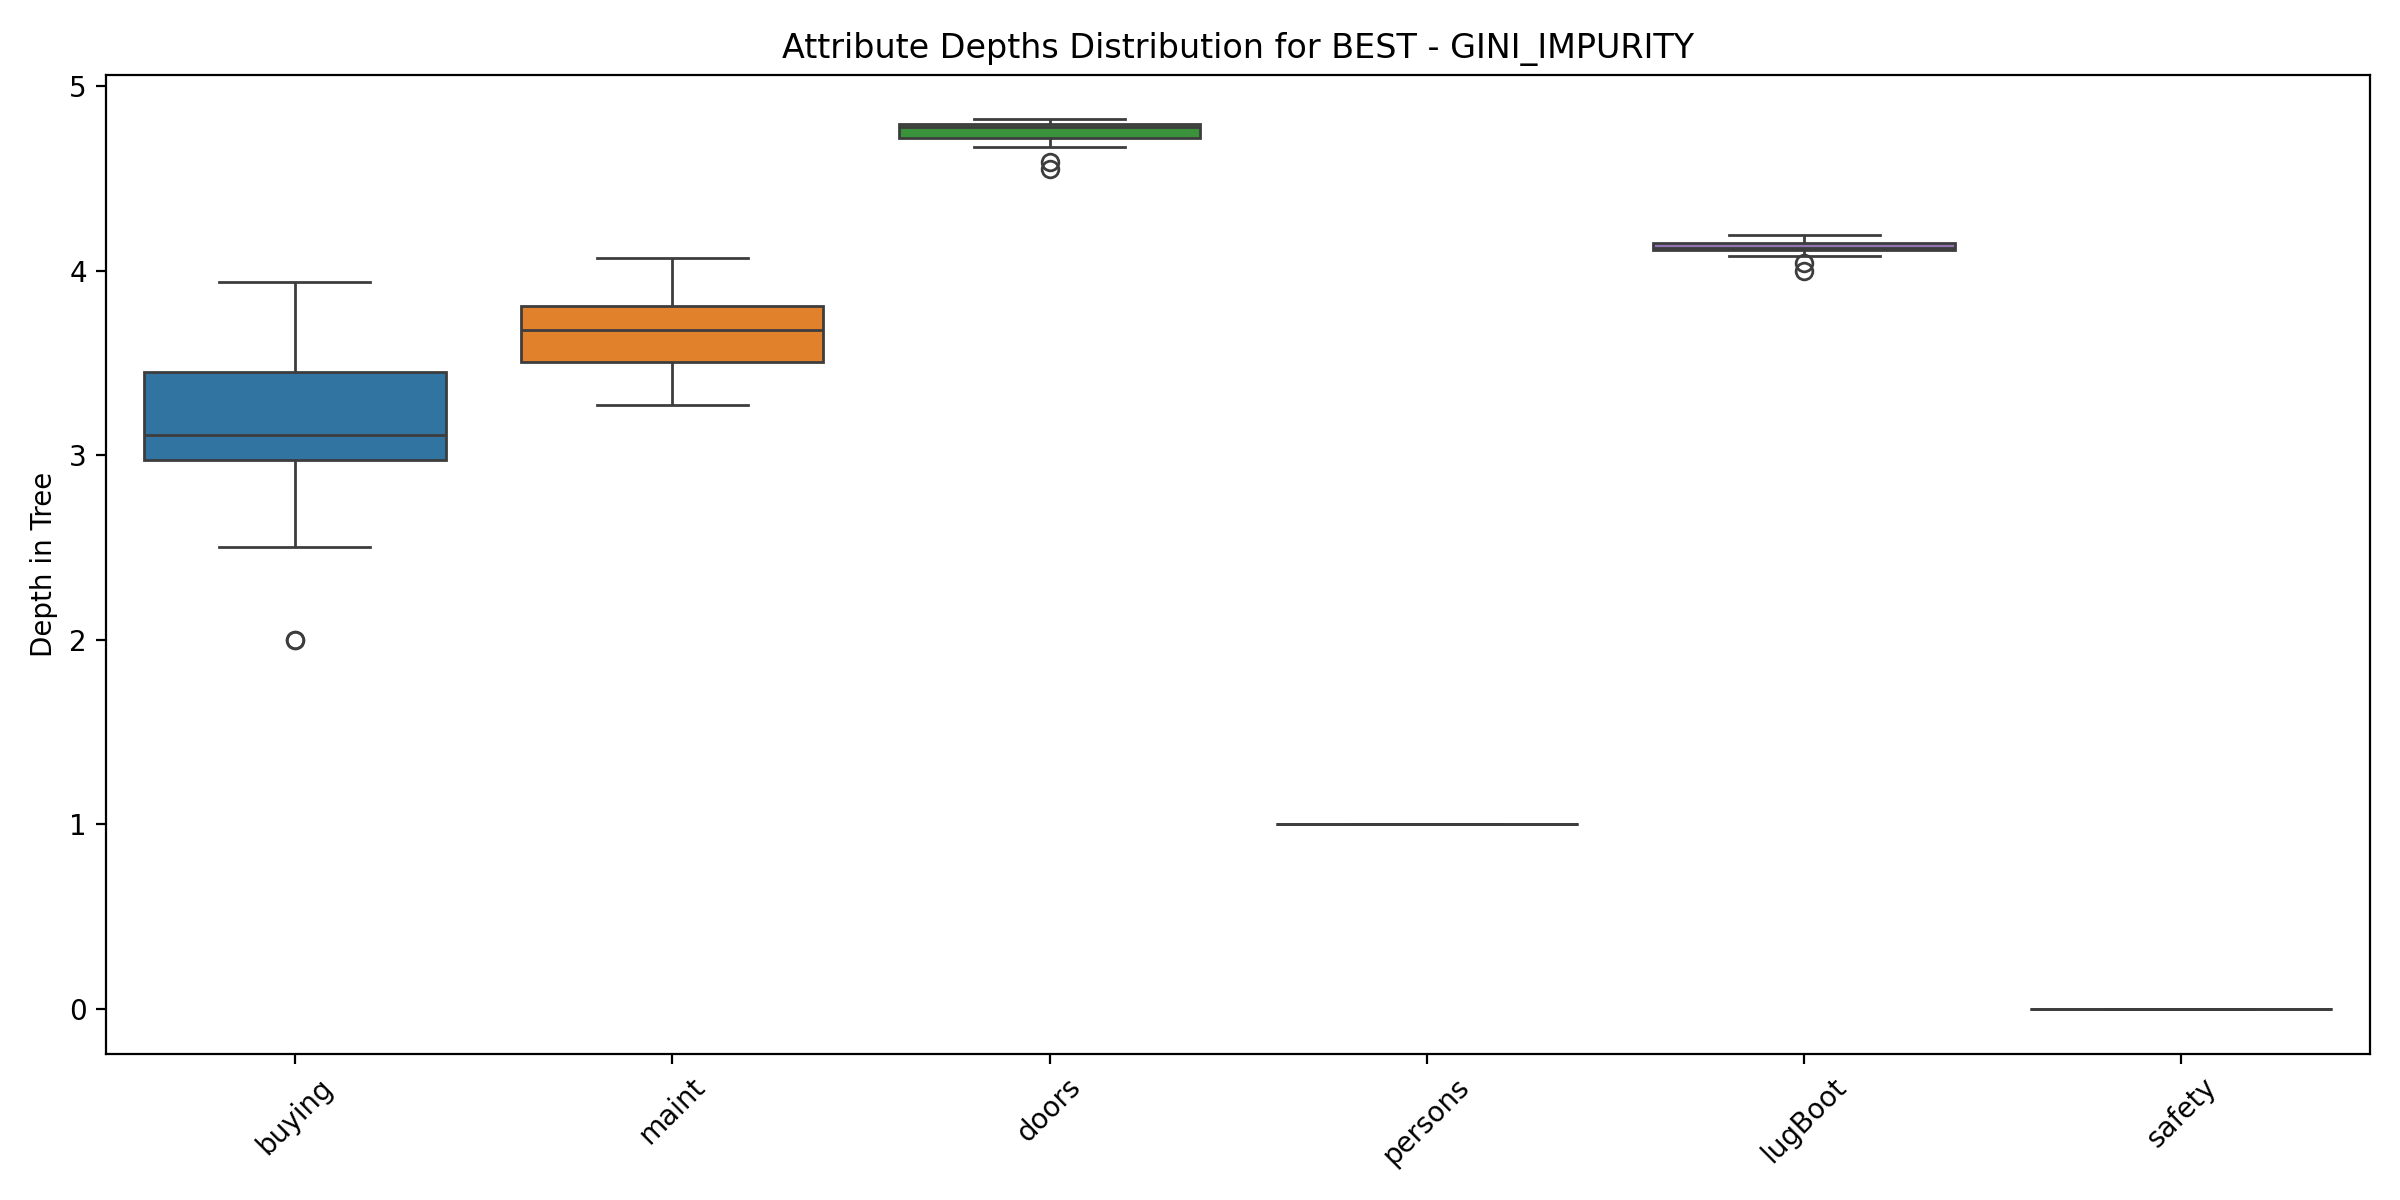
\includegraphics[width=0.9\textwidth]{plots/attribute_depths_BEST_GINI_IMPURITY.png}
    \caption{Distribution of attribute depths for BEST strategy with GINI IMPURITY metric.}
    \label{fig:attr-best-gini}
\end{figure}
\newpage

\begin{figure}[H]
    \centering
    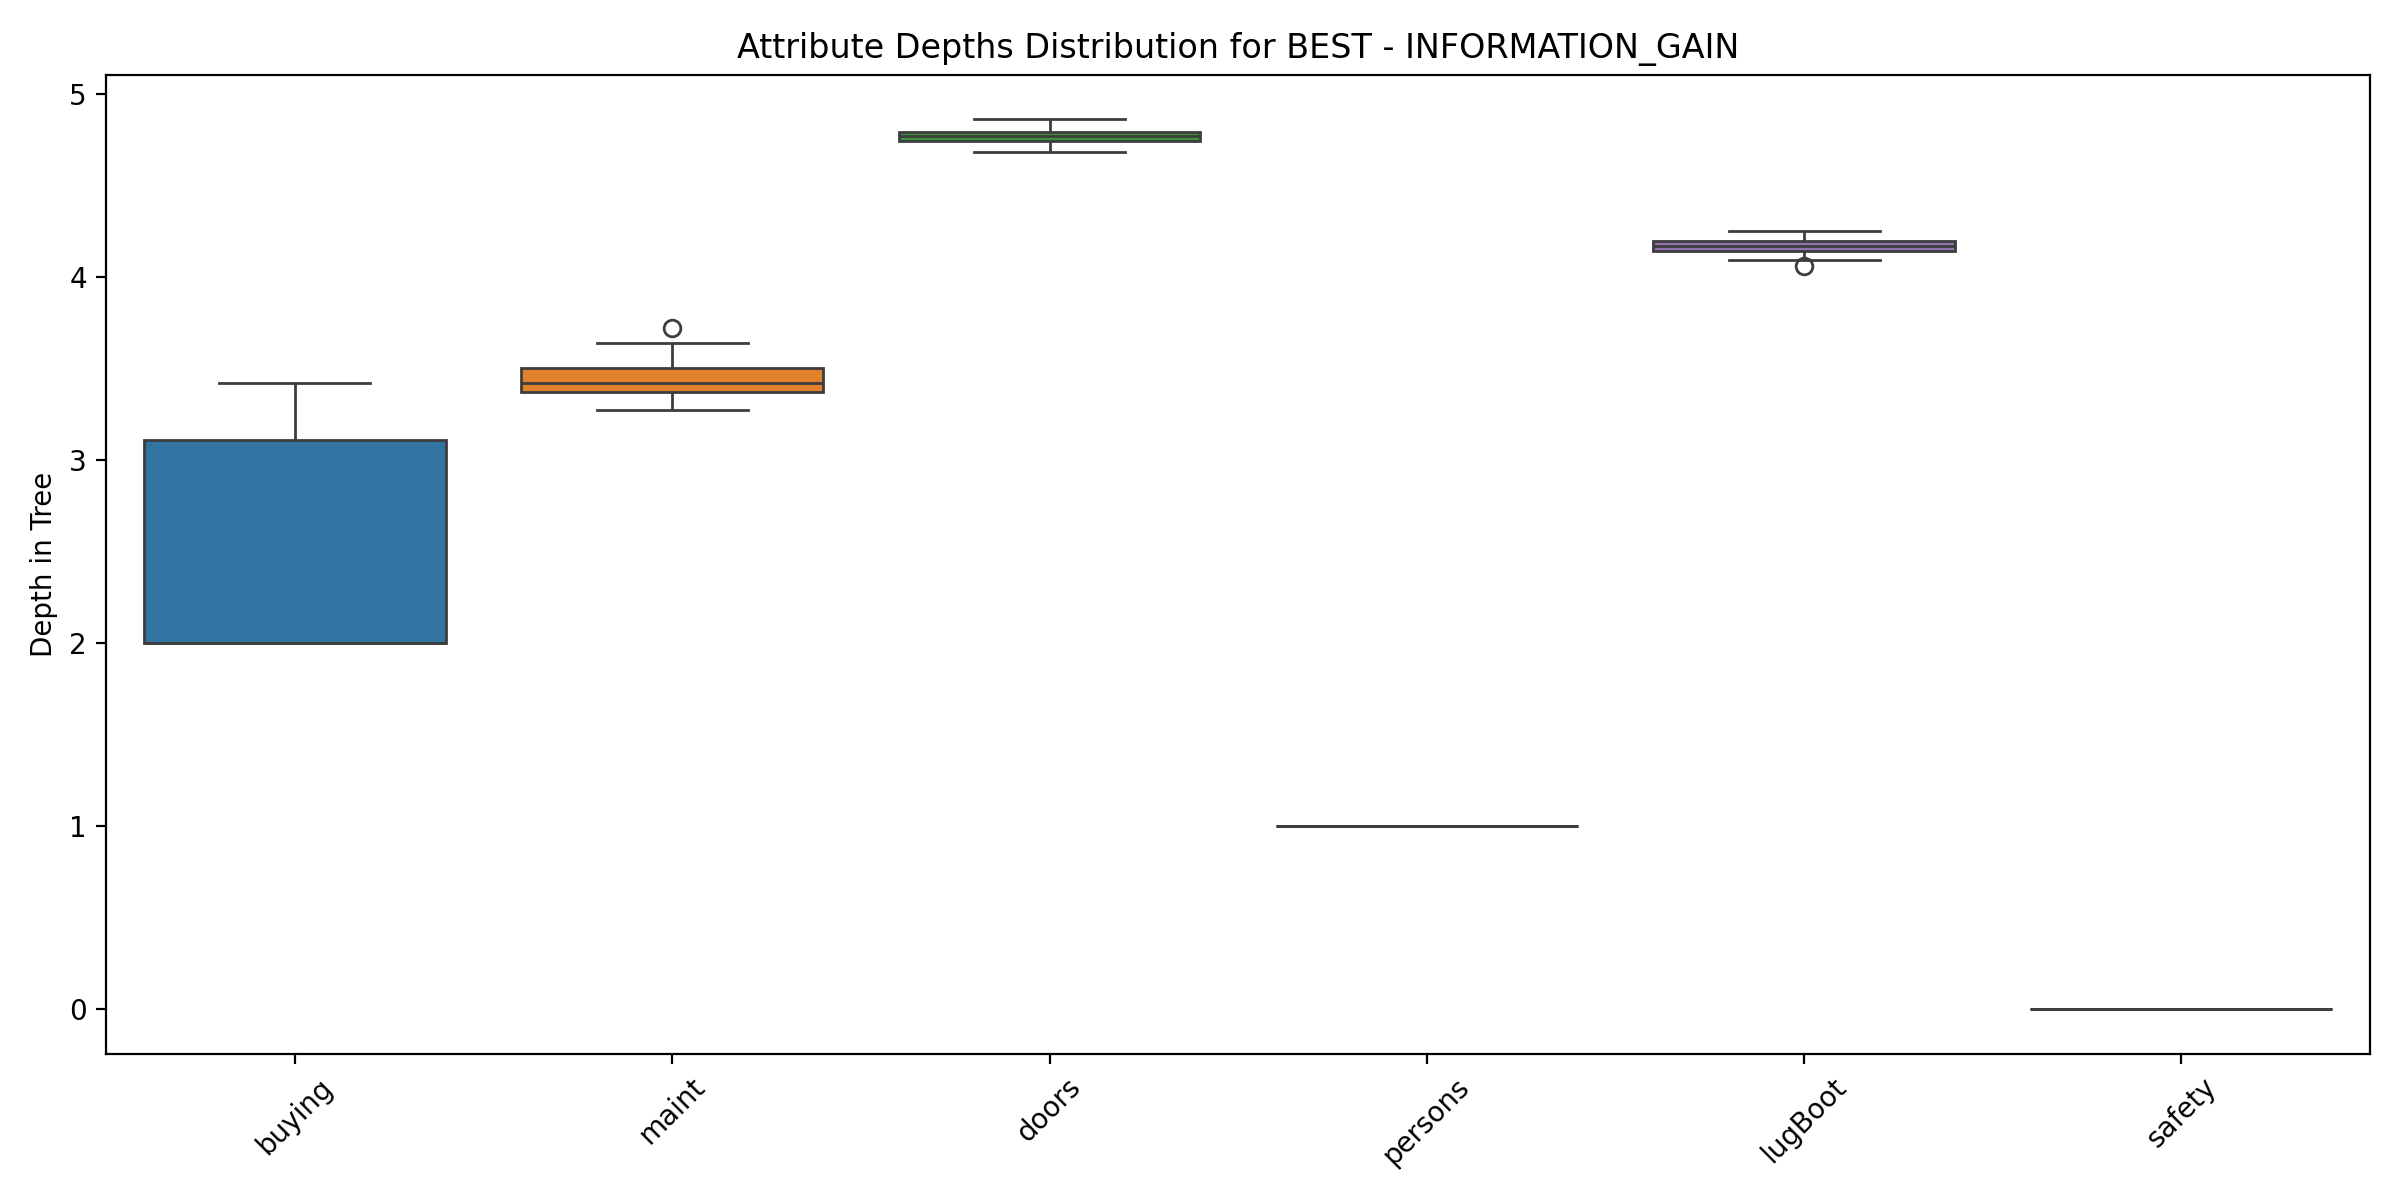
\includegraphics[width=0.9\textwidth]{plots/attribute_depths_BEST_INFORMATION_GAIN.png}
    \caption{Distribution of attribute depths for BEST strategy with INFORMATION GAIN metric.}
    \label{fig:attr-best-ig}
\end{figure}
\newpage

\begin{figure}[H]
    \centering
    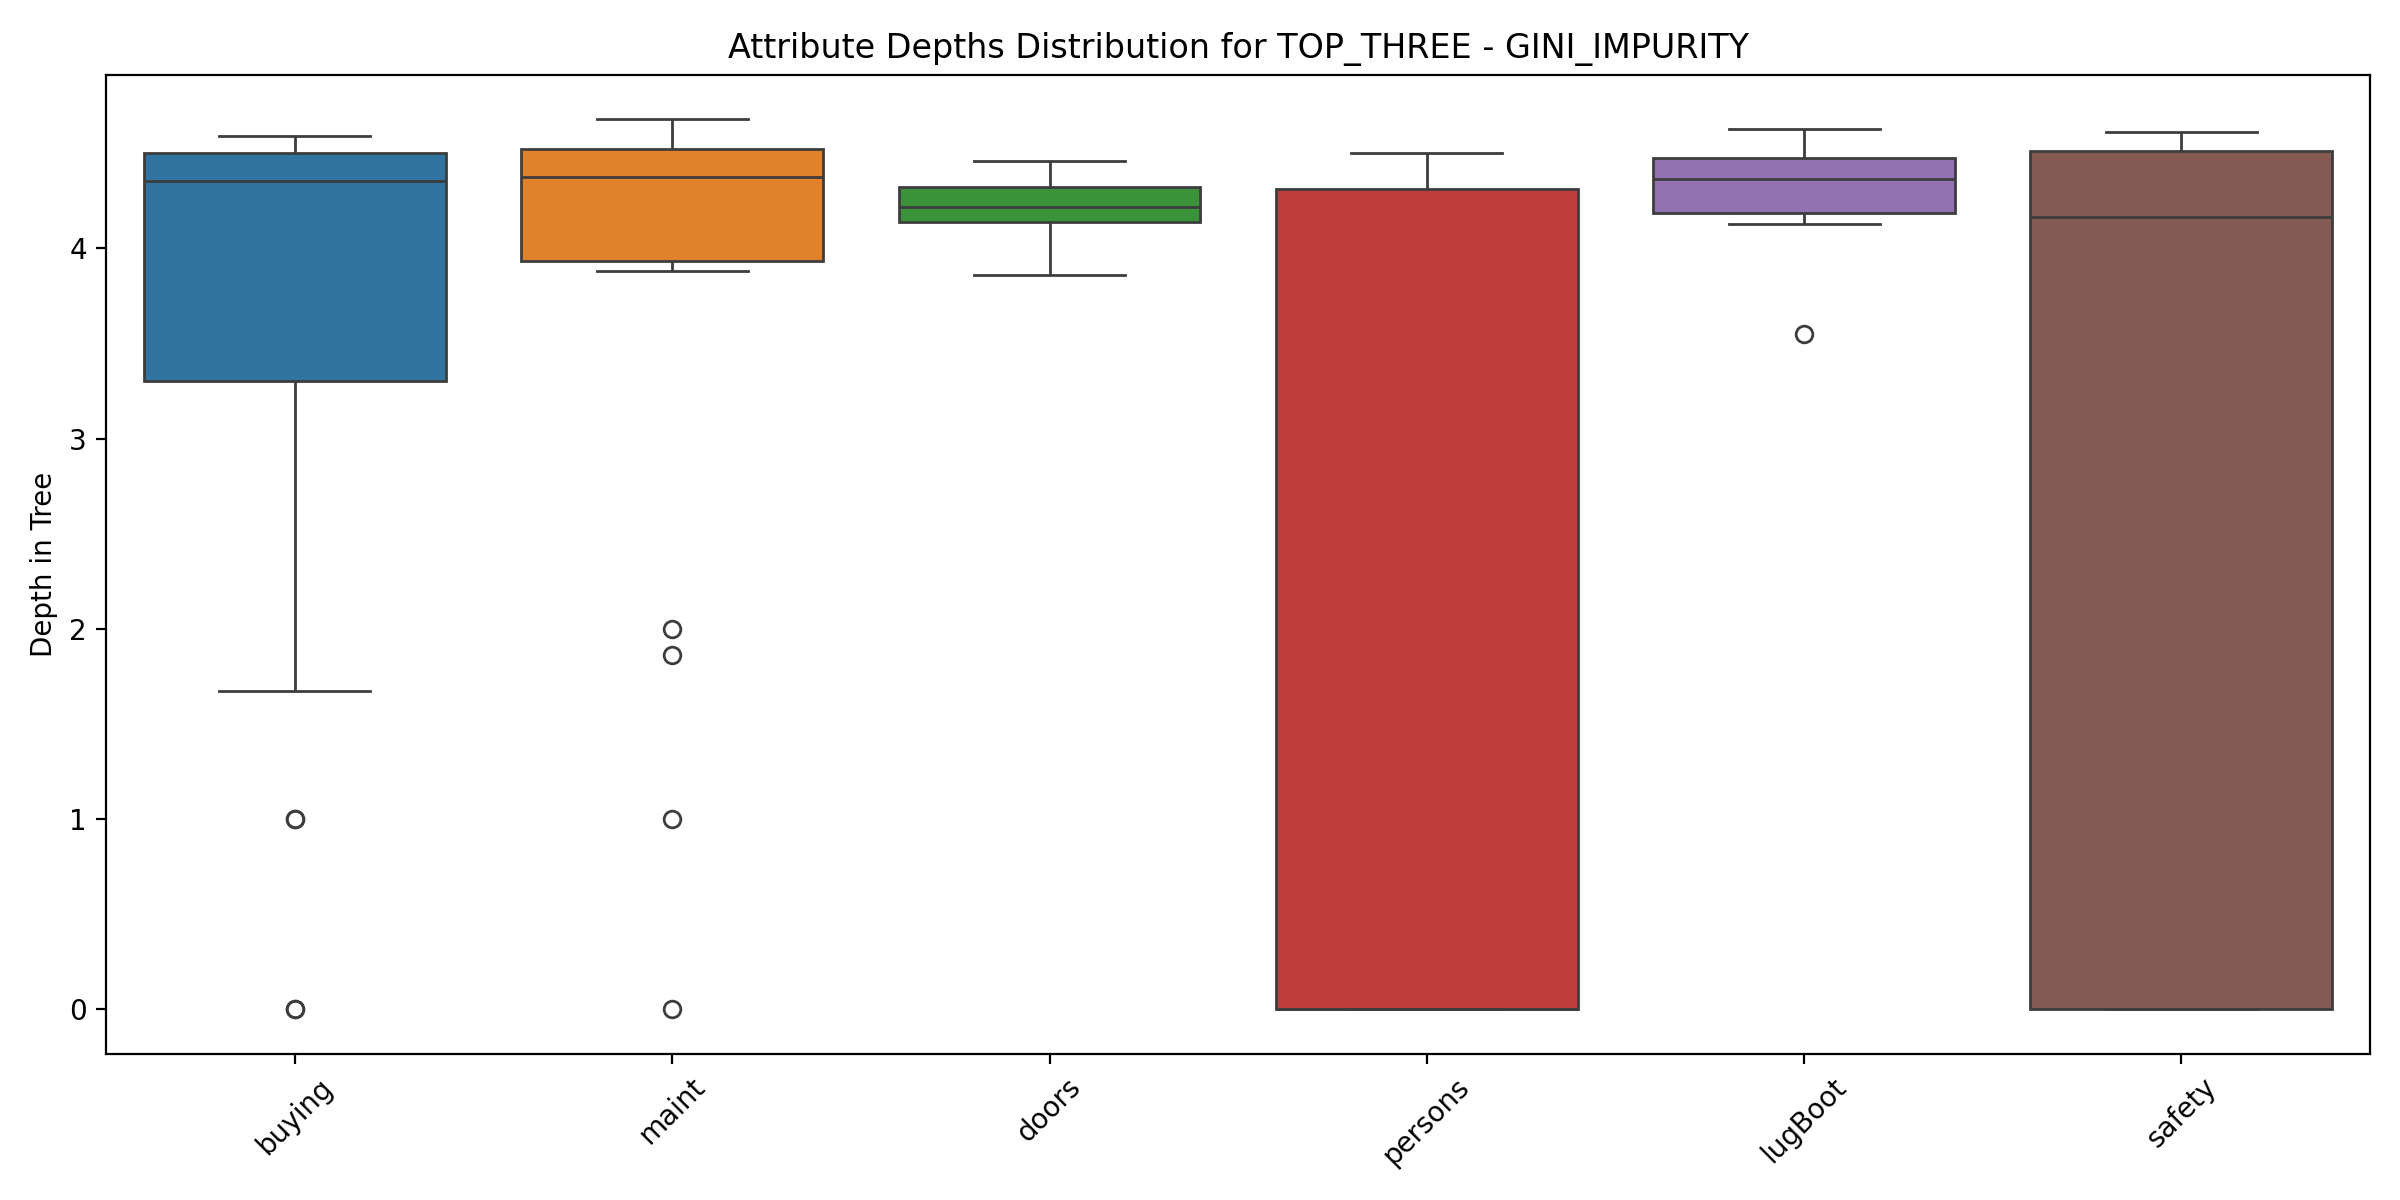
\includegraphics[width=0.9\textwidth]{plots/attribute_depths_TOP_THREE_GINI_IMPURITY.png}
    \caption{Distribution of attribute depths for TOP THREE strategy with GINI IMPURITY metric.}
    \label{fig:attr-top3-gini}
\end{figure}
\newpage

\begin{figure}[H]
    \centering
    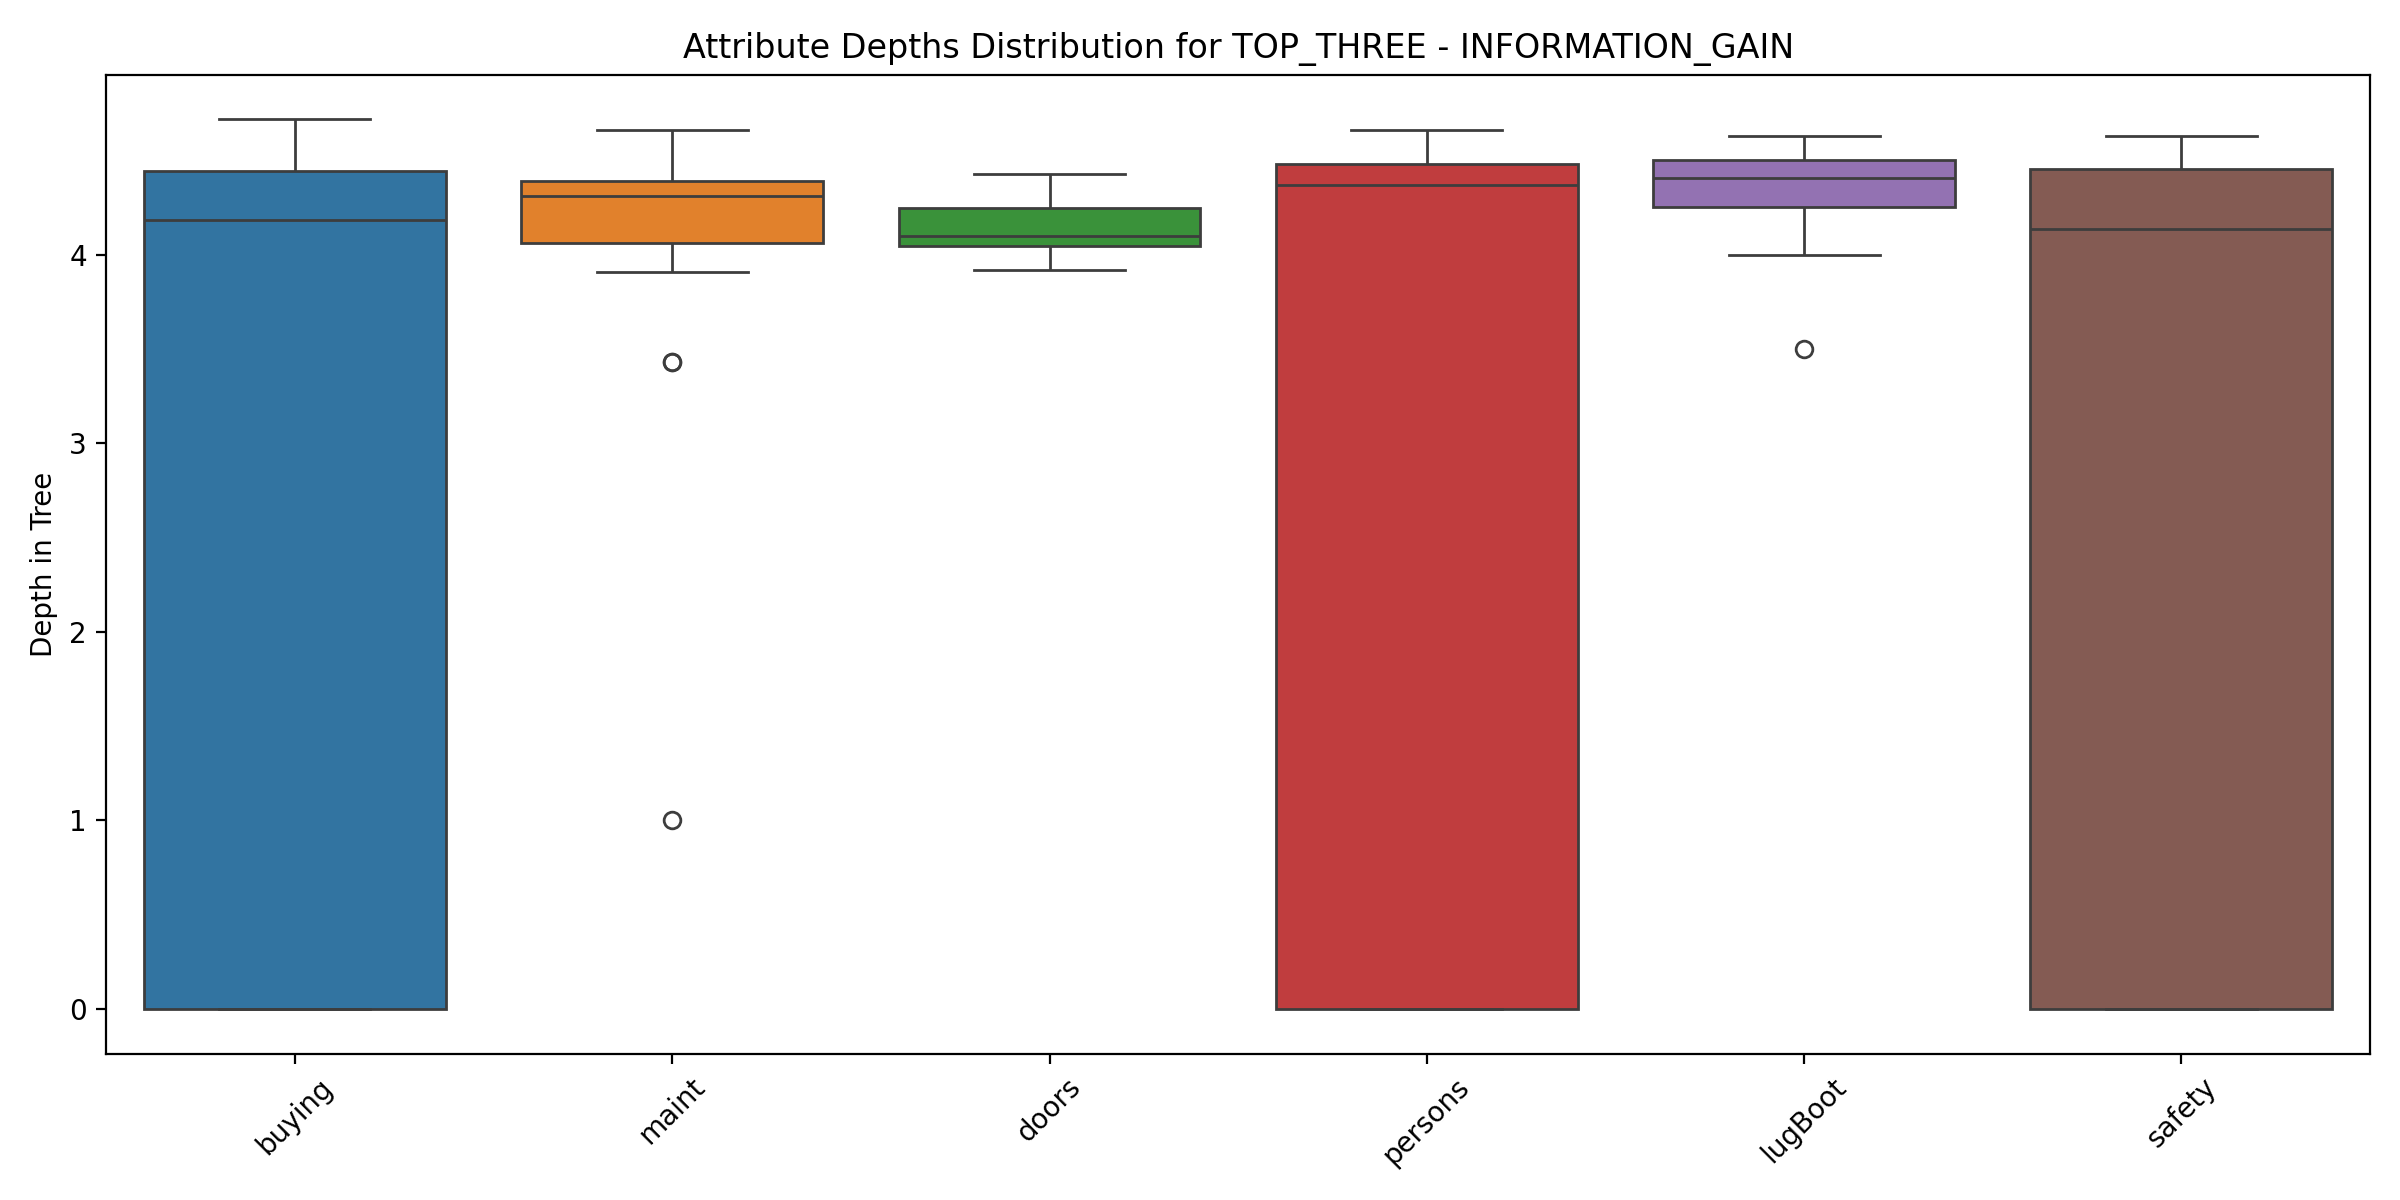
\includegraphics[width=0.9\textwidth]{plots/attribute_depths_TOP_THREE_INFORMATION_GAIN.png}
    \caption{Distribution of attribute depths for TOP THREE strategy with INFORMATION GAIN metric.}
    \label{fig:attr-top3-ig}
\end{figure}
\newpage

% Training Metrics (Individual plots)
\subsection{Training Metrics Analysis}

\begin{figure}[H]
    \centering
    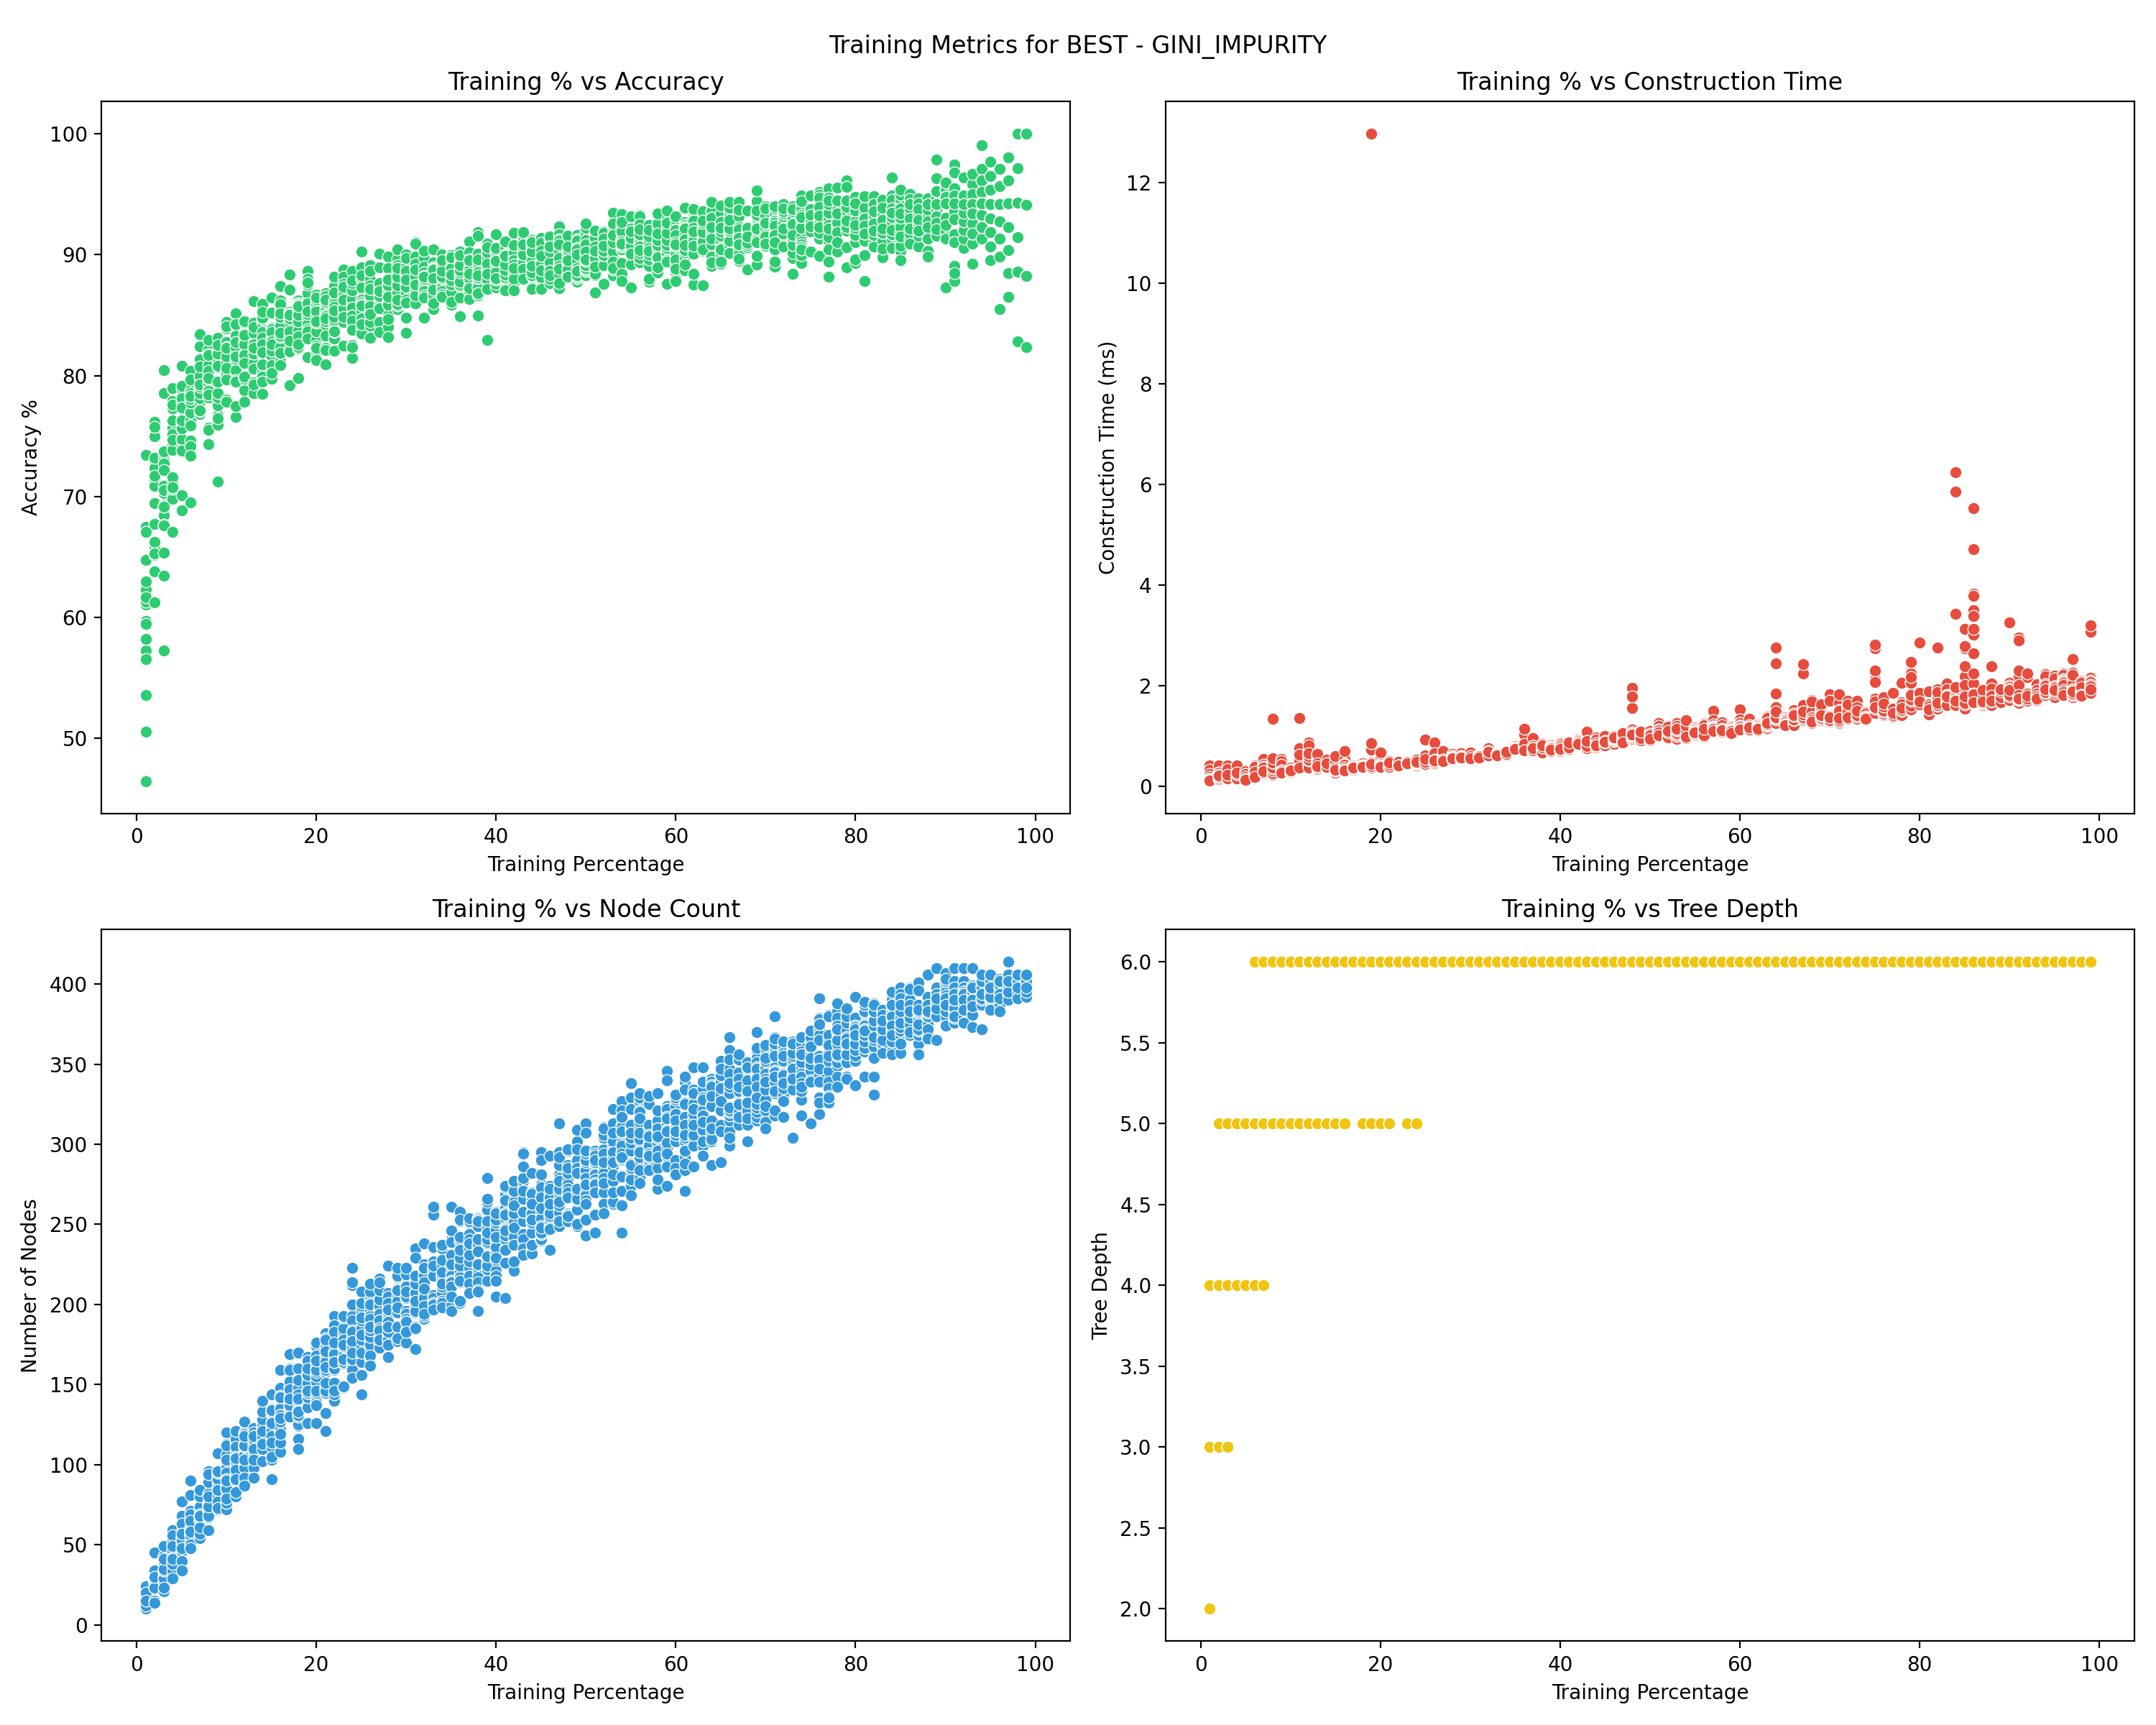
\includegraphics[width=0.9\textwidth]{plots/training_metrics_BEST_GINI_IMPURITY.png}
    \caption{Training metrics for BEST strategy with GINI IMPURITY metric showing relationships between training percentage and various performance measures.}
    \label{fig:training-best-gini}
\end{figure}
\newpage

\begin{figure}[H]
    \centering
    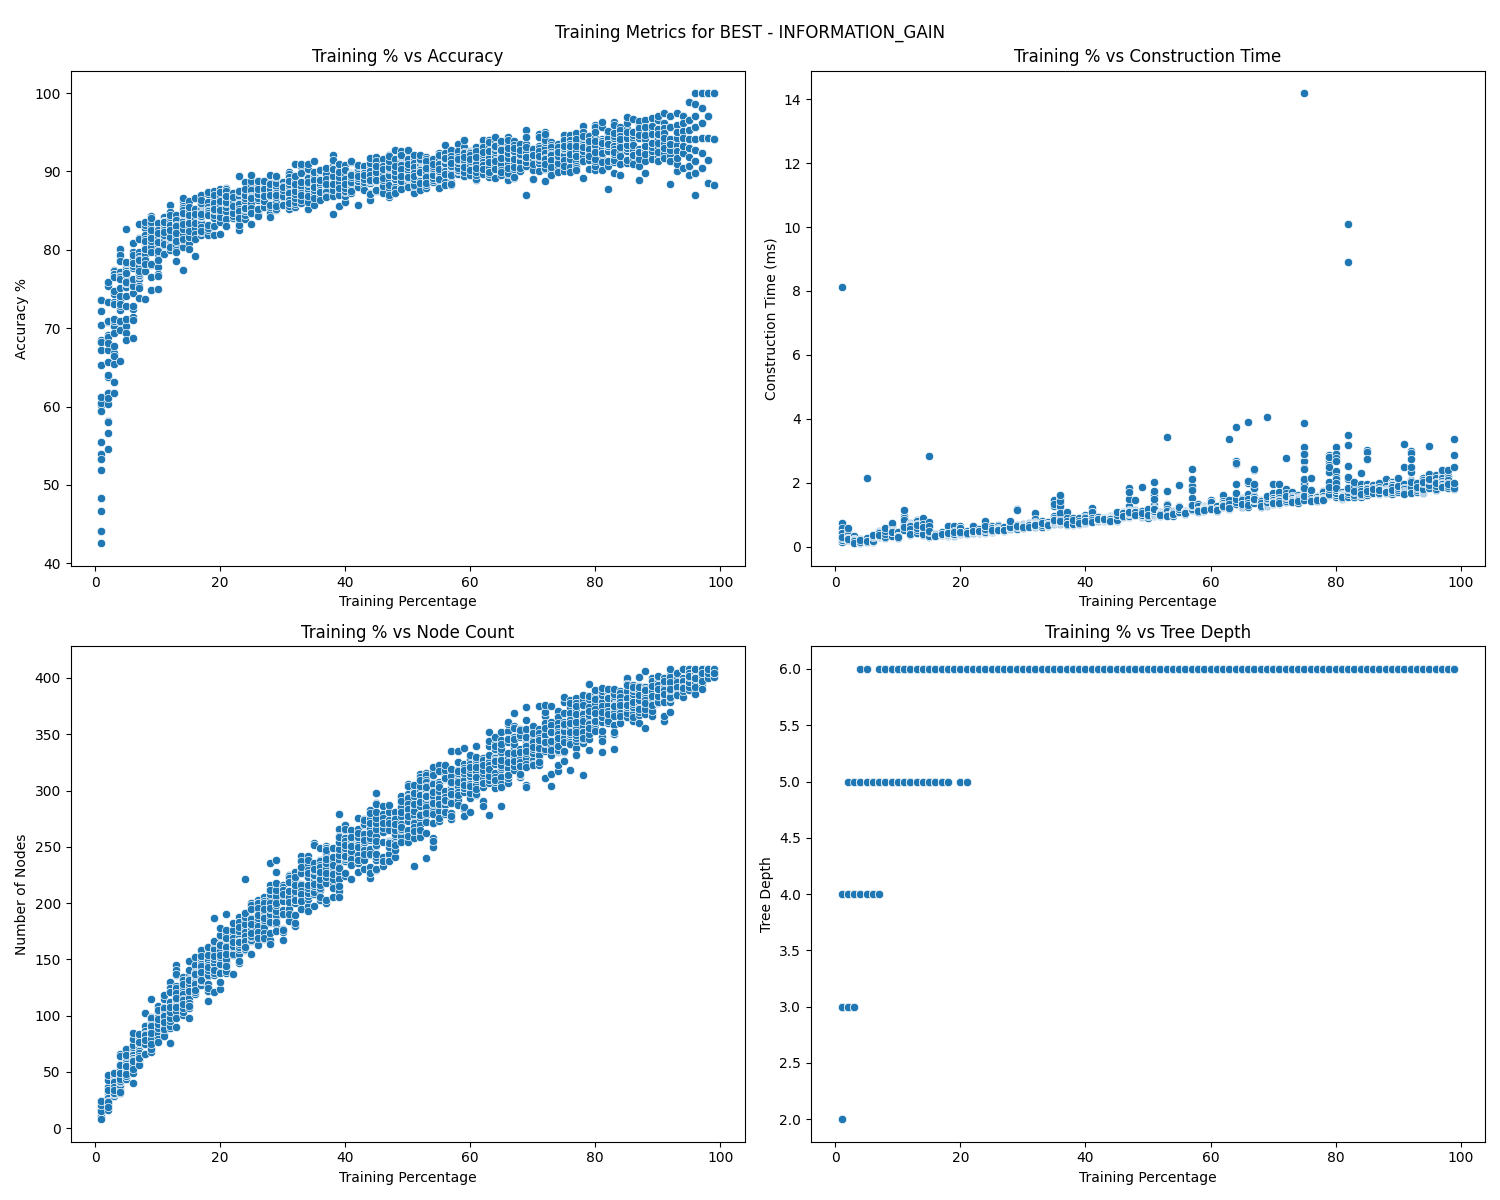
\includegraphics[width=0.9\textwidth]{plots/training_metrics_BEST_INFORMATION_GAIN.png}
    \caption{Training metrics for BEST strategy with INFORMATION GAIN metric showing relationships between training percentage and various performance measures.}
    \label{fig:training-best-ig}
\end{figure}
\newpage

\begin{figure}[H]
    \centering
    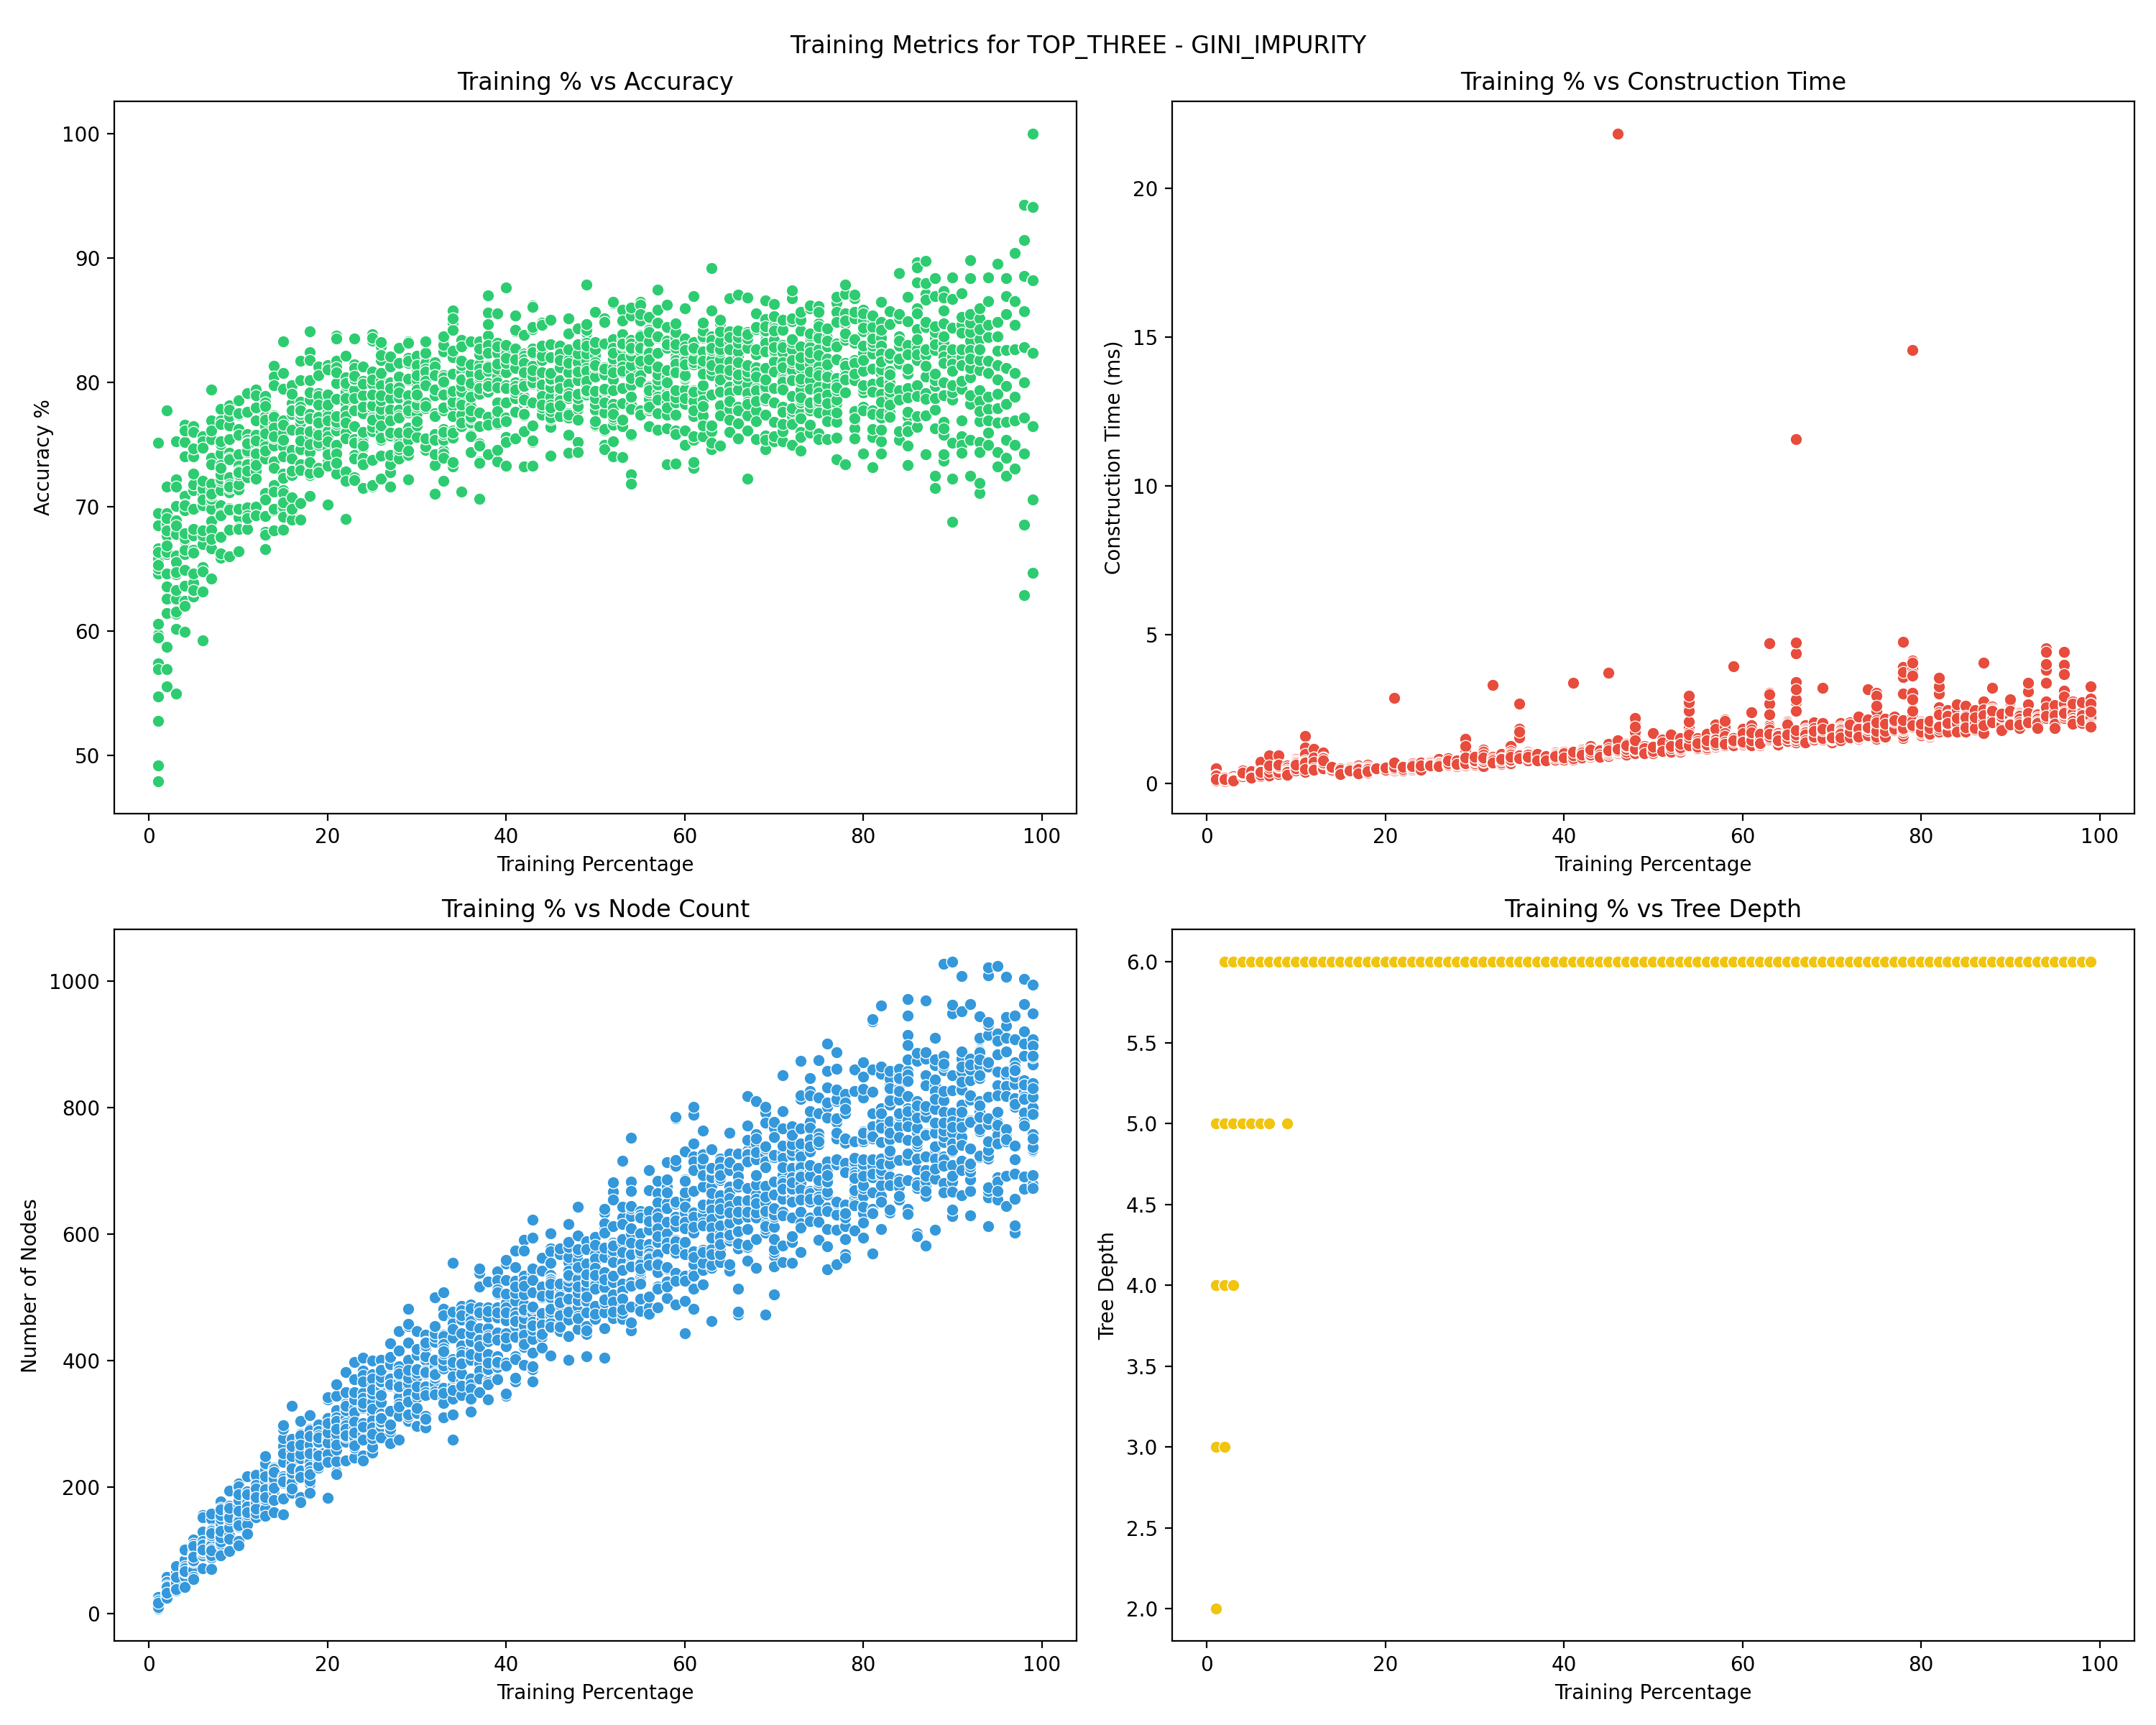
\includegraphics[width=0.9\textwidth]{plots/training_metrics_TOP_THREE_GINI_IMPURITY.png}
    \caption{Training metrics for TOP THREE strategy with GINI IMPURITY metric showing relationships between training percentage and various performance measures.}
    \label{fig:training-top3-gini}
\end{figure}
\newpage

\begin{figure}[H]
    \centering
    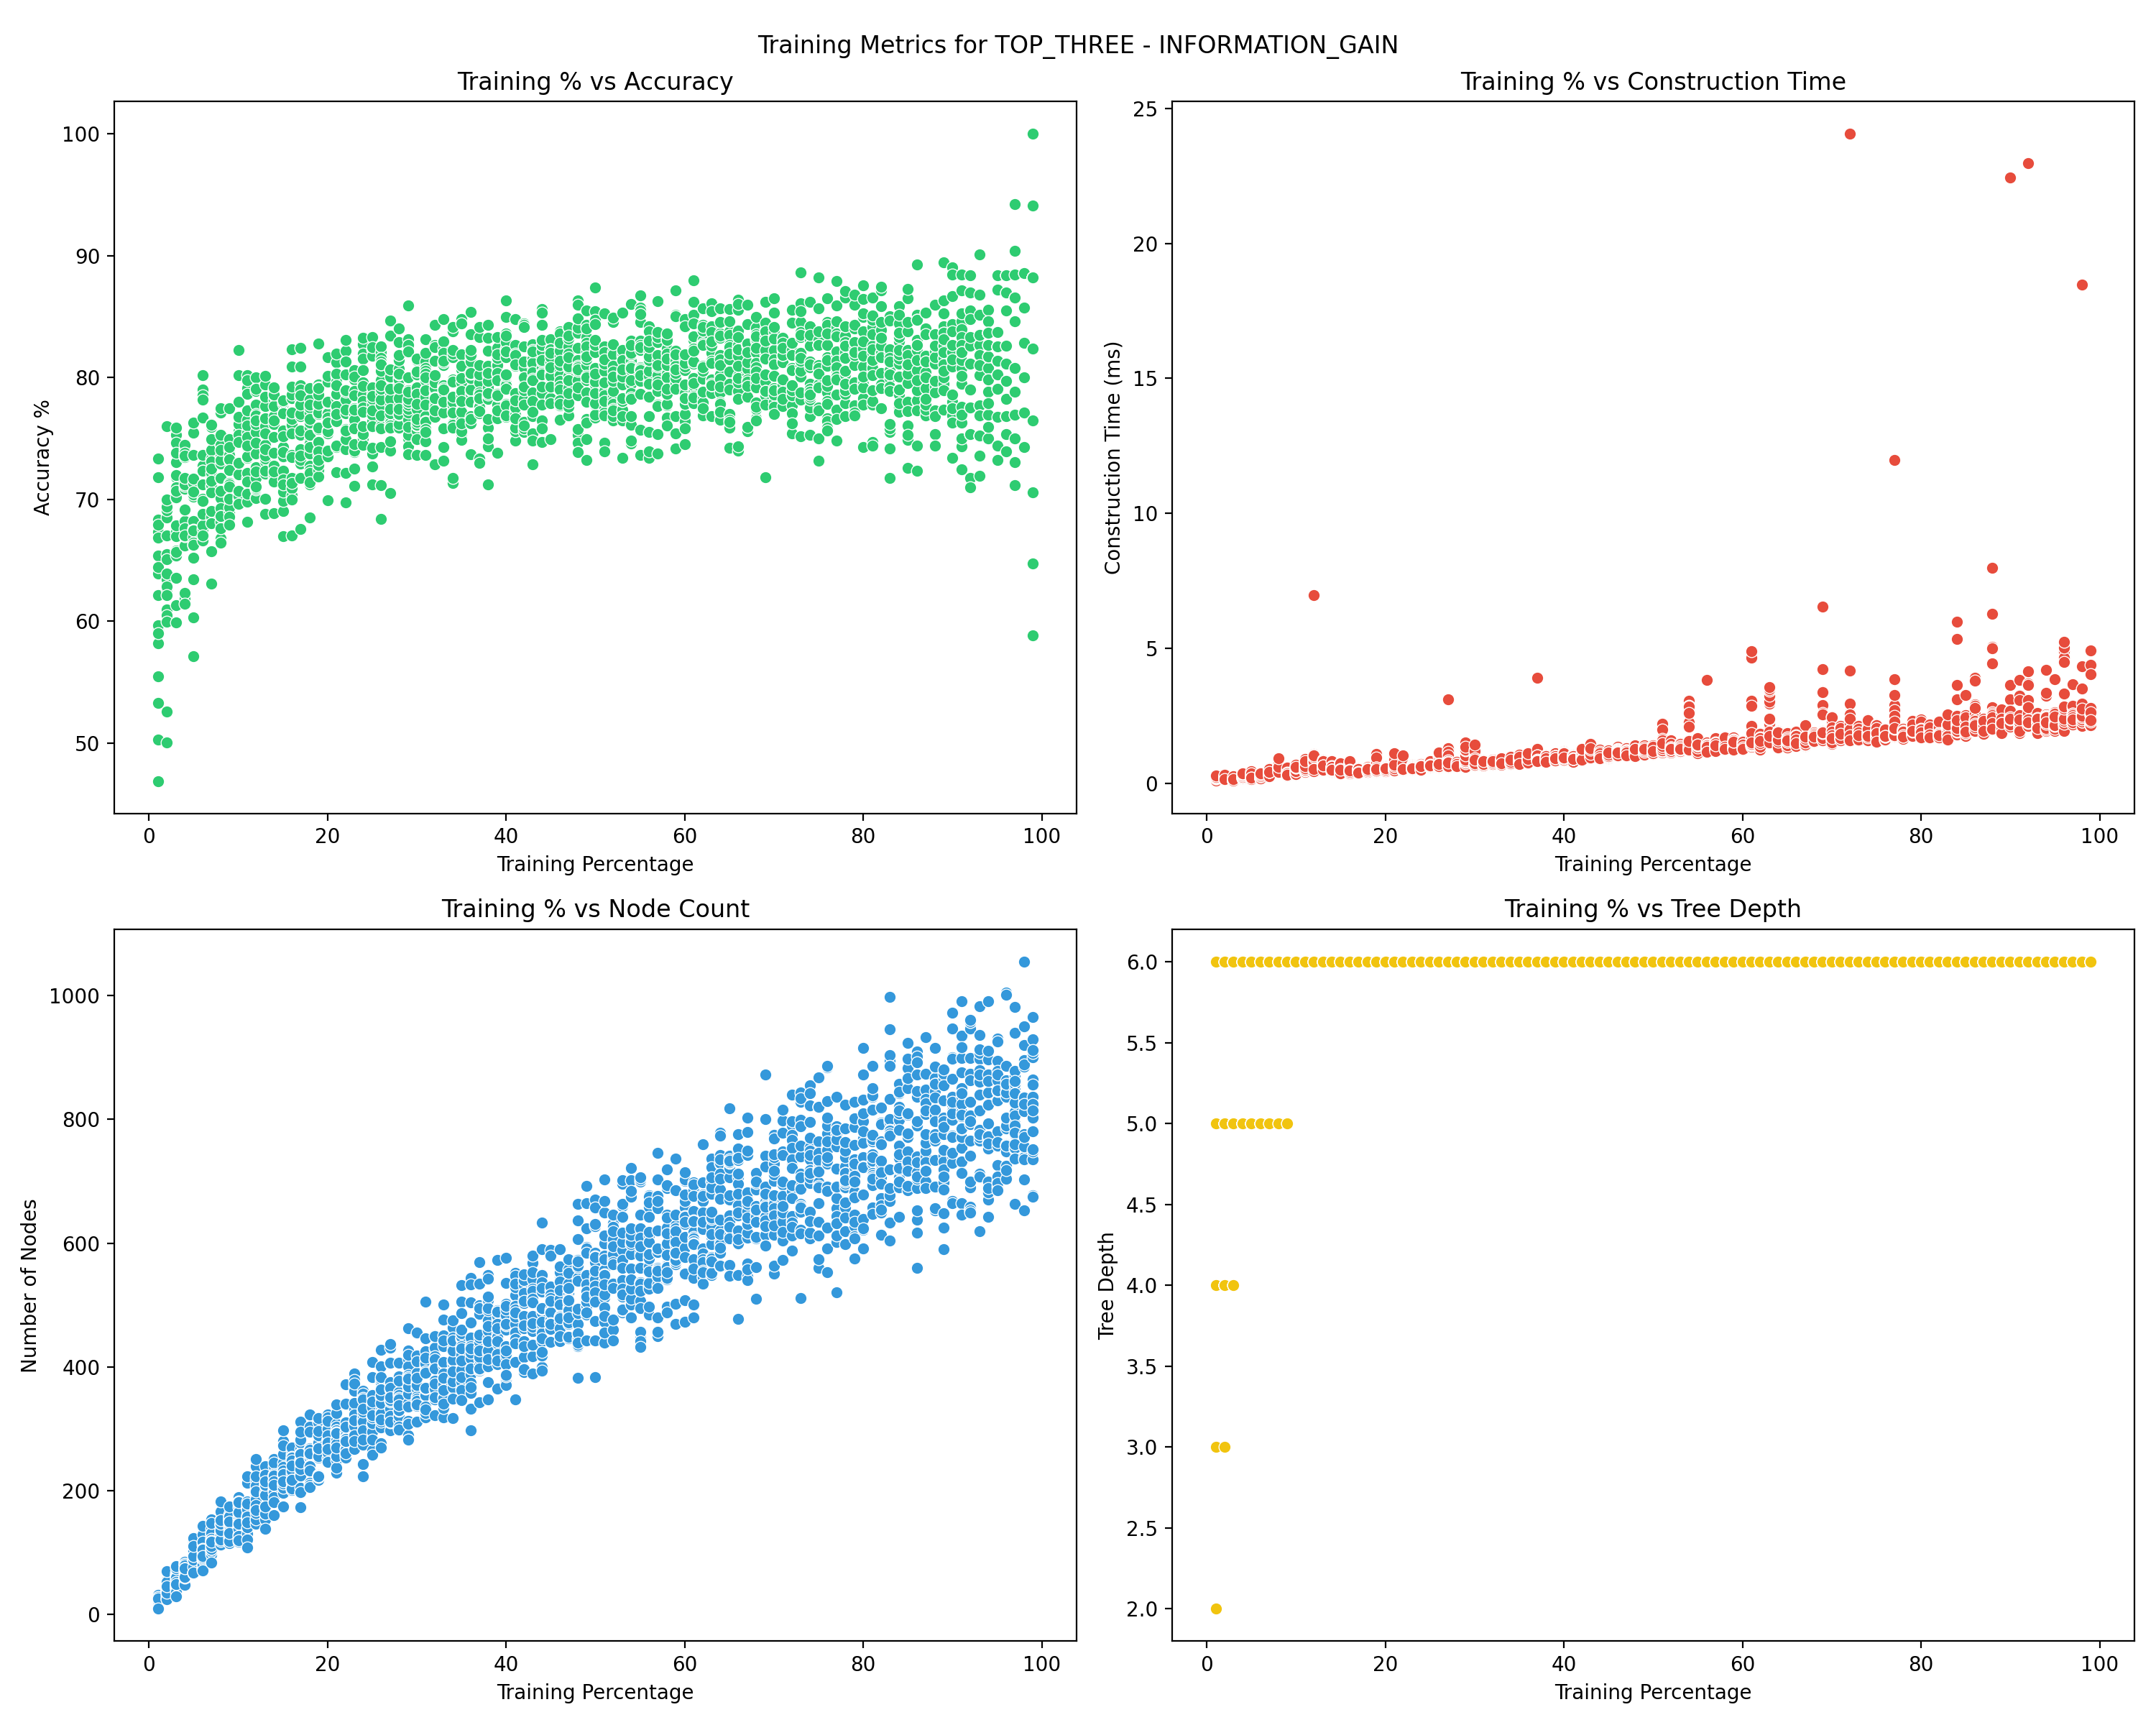
\includegraphics[width=0.9\textwidth]{plots/training_metrics_TOP_THREE_INFORMATION_GAIN.png}
    \caption{Training metrics for TOP THREE strategy with INFORMATION GAIN metric showing relationships between training percentage and various performance measures.}
    \label{fig:training-top3-ig}
\end{figure}

\end{document}
